\documentclass[12pt]{article}
\usepackage[margin=1.5cm]{geometry}
\usepackage{parskip}
\usepackage{amsmath}
\usepackage{amssymb}
\usepackage{amsfonts}
\usepackage{enumitem}
\usepackage{graphicx}
\usepackage{stmaryrd}
\graphicspath{ {./images/} }


\begin{document}
\begin{enumerate}[label=(\alph*)]
  \item
    The general framework is as follows: taking the big union/intersection over the predecessors/successors of a node, and then removing `kill' and `gen' sets, either of the successors/predecessors or of the node itself.

    Whether we take the predecessors/successors corresponds to forwards/backwards dataflow analysis respectively, and the location of the `kill' and `gen' sets corresponds to when the data is needed for transformation.

    For LVA, we get the following data-flow equation:

    \[
      live(n) = \left(\bigcup_{s \in succ(n)} live(s)\right) \setminus kill(n) \cup gen(n)
    .\] 

    And for AVAIL, we get the following data-flow equation:

    \[
      avail(n) = \left(\bigcap_{p \in pred(n)} avail(p) \setminus kill(p) \cup gen(p) \right)
    .\] 

    Here, we see that LVA takes the big union over successors, so it is a backwards data flow, and we use the kill and gen sets of the node itself, so we need the analysis before each node, not after.

    AVAIl takes the big intersection over predecessors, so it is a forwards data flow, and we use the kill and gen sets of the predecessors, so we need the analysis before each node also (since we flip the dierction of the analysis).

  \item
    Liveness analysis can be used to identify both dead code and uninitialised variables.

    When we write to a variable that is not live at that point, we know that it will have no effect on the IO behaviour of the program, so we can remove it.

    When a variable is live at declaration, we know that it might be used before it is first defined.

  \item
    Semantic expression availability refers to whether an expression is available in every possible execution of a program. Syntactic expression availability refers to whether an expression in every path through a program, including those that do not correspond to any execution of the program.

    For example:

\begin{verbatim}
x = rand()
if ((x+1) * (x+1) == 0) {
  a = SomeExpr
}
if (x*x + 2*x + 1 != 0) {
  b = SomeExpr
}
c = SomeExpr
\end{verbatim}

We see that \texttt{SomeExpr} is available at the definition of \texttt{c}, since one of the \texttt{if} statements will always be entered, but there exists a path through the program that enters neither (even if it is not possible), so \texttt{SomeExpr} is not syntactically available at the definition of \texttt{c}.

The analysis is still safe, with respect to the usual transformations, since syntactic availability is a subset of semantic availability, so we never consider an expression available if it is not, we only consider some expressions not available (even though they might be). This means that if we want to do something like common subexpression elimination, we will not try and use the result of an expression that has not been computed.

\item
  It might be useful to run copy propagation after this transformation because common subexpression elimination can produce long chains of unnecessary copies to use the pre-computed results, so copy propagation allows the number of these copies to be reduced.

\item
  We perform LVA, assuming that \texttt{func} does not have access to the variables:

\begin{verbatim}
a = func(1); {}
b = func(2); {a}
c = a * b;   {a,b}
print(b,c);  {a,b,c}
d = c - a;   {a,c}
print(a,d);  {a,c,d}
e = d - 1;   {a,c,d}
b = c + a;   {a,c,e}
d = e + b;   {b,e}
print(d,e);  {b,d,e}
f = e-5;     {b,e}
print(b,f);  {b,f}
return;      {}
\end{verbatim}

This gives us the following clash graph:

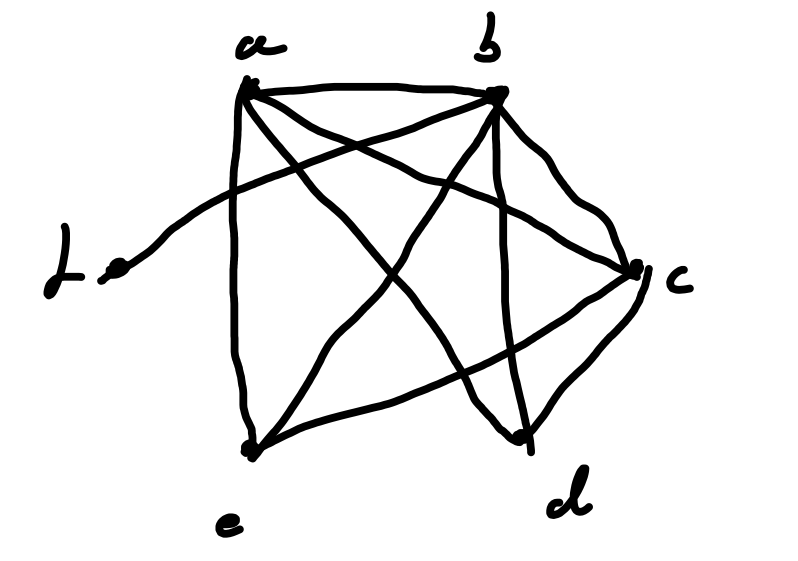
\includegraphics[scale=0.3]{clashgraph}

We see here that we can perform the following allocation, that does not violate the clash graph:

\begin{verbatim}
a = r1
b = r2
c = r3
d = r4
e = r4
f = r1
\end{verbatim}

This takes 4 registers, so five registers are definitely sufficient to hold its variables.

The minimum number of registers is also 4, since the clash graph contains subgraph \texttt{a,b,c,d}, which is the graph $K_4$, which means we require at least 4 colours to colour the clash graph, which we have done.






        
\end{enumerate}
\end{document}
